% !TEX root=/home/tavant/these/manuscript/src/manuscript.tex


\section*{Plasma models and simulations}
\label{sec-simulations}
\addcontentsline{toc}{section}{Plasma models and simulations}

The plasma is the state of mater were the internal energy is high enough to ionize the atoms.
Depending of the pressure, energy, and time scale, different models are better to describe the plasma.
There are mainly two distinct models.
The first is the \emph{kinetic} description of the species of the plasma, via the Boltzmann equation.
The second uses a \emph{fluid} description of the species, by means of moments.
% 
% \begin{figure}[hbtp]
%   \centering
%   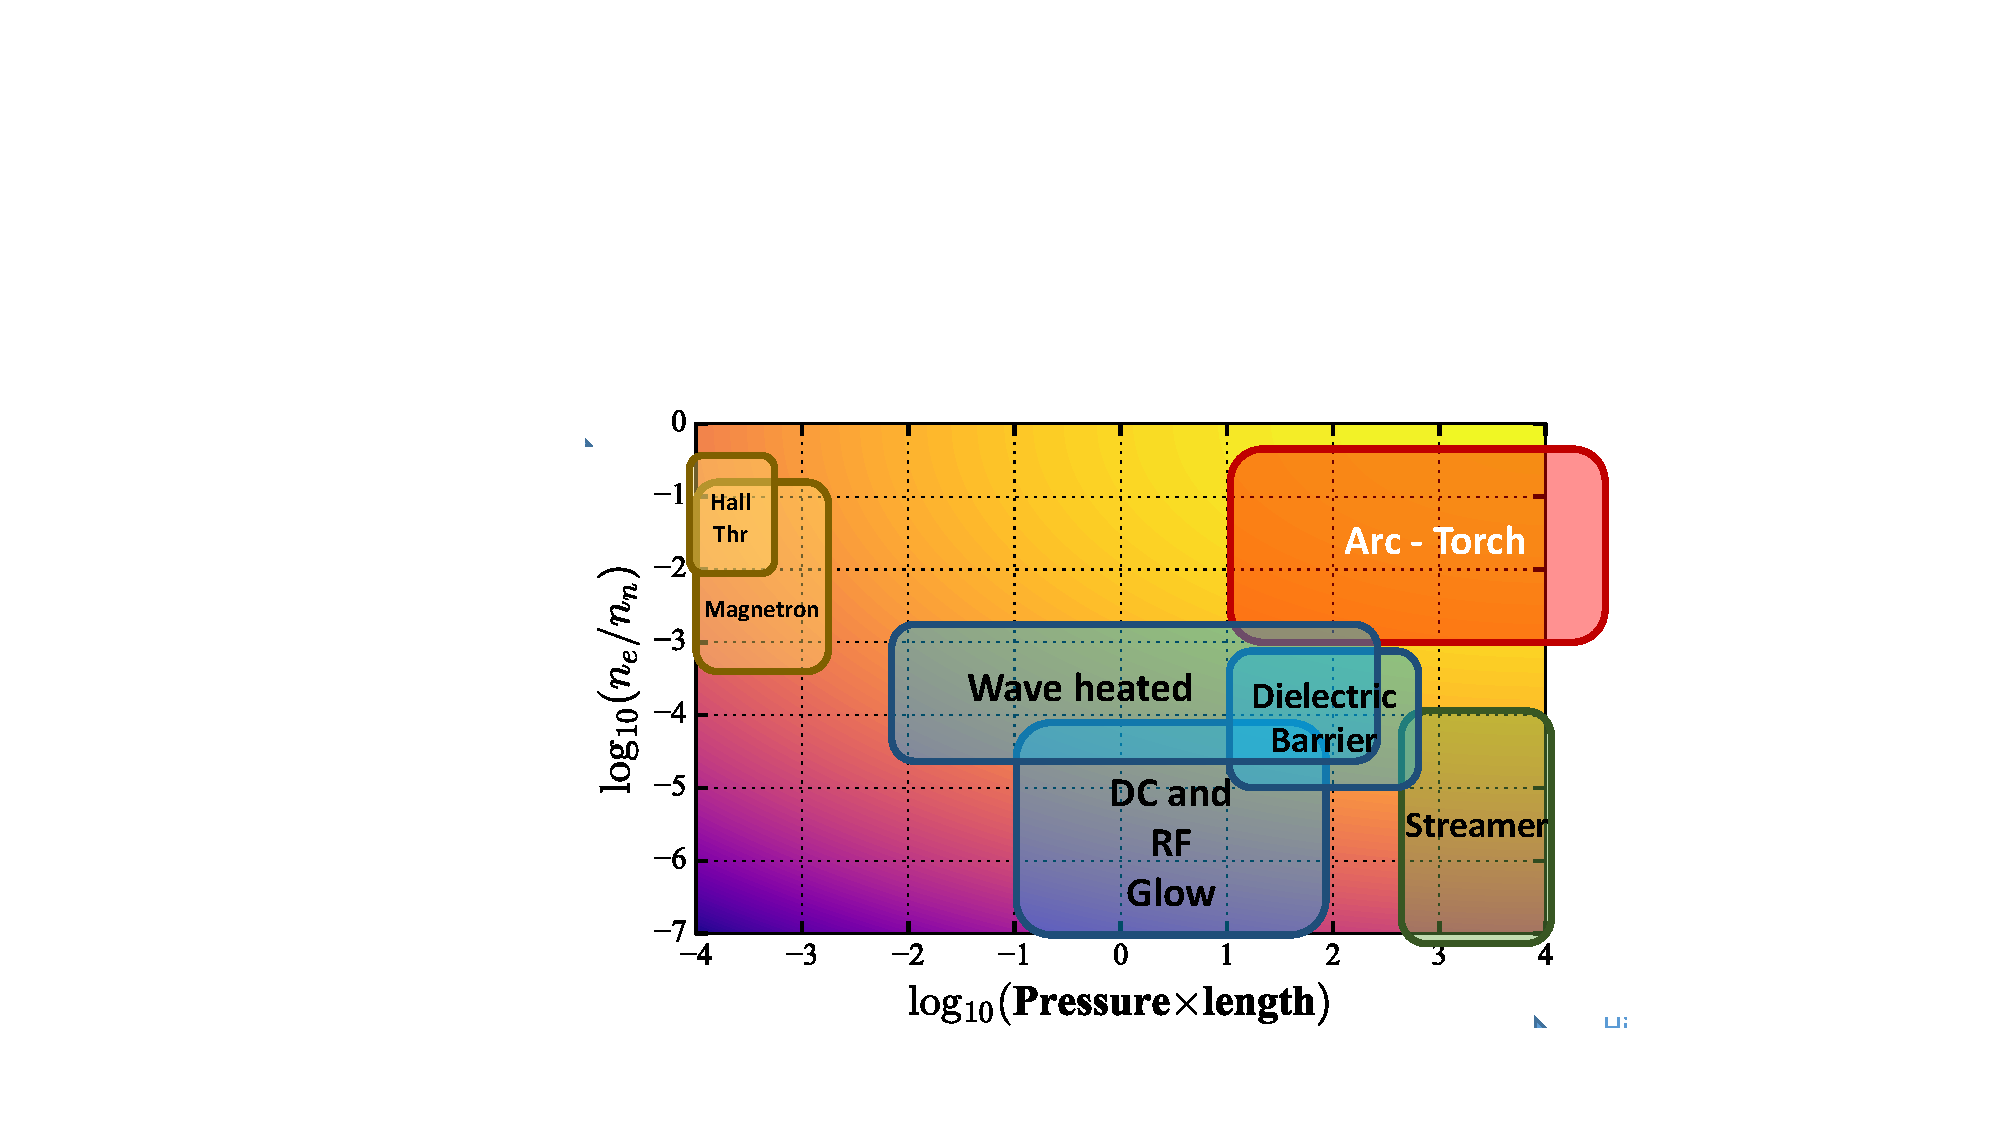
\includegraphics[width=\defaultwidth]{Chart}
%   \caption{}
%   \label{fig-chart}
% \end{figure}


\paragraph{Boltzmann equation \\}
The Boltzmann equation in \cref{eq-boltzmann} describes the evolution of the particles (atoms, ions and electrons) in the phase space.
The phase space is the set of all possible position $\vect{x}$ and velocity $\vect{v}$ that can be attained by a particle.
The evolutions in the phase space are due to forces, diffusion and collisions.

\begin{equation} \label{eq-boltzmann}
\deriv{f}{t}  + \vect{v} \cdot \grad_{\vect{x}} f + \vect{F} \cdot  \grad_{\vect{v}} f = \deriv{f}{t} \at{\rm coll}
\end{equation}
where $f$ is the distribution function of the particle at $\vect{x}, \vect{v}$, and $\deriv{f}{t}\mid_{\rm coll}$ denotes the effects of the collisions, $\grad$ is the gradient in both the positions (subscript $\vect{x}$) and the velocities (subscript $\vect{v}$)  and $\vect{F}$ is the force applied to the particle.
In the general electro-magnetic case,
\begin{equation*} \label{eq-forceEM}
  \vect{F} =  q \vect{E} + q \vect{v} \times \vect{B}
\end{equation*}
with $q$ the particle charge, $\vect{E}$ the electric field, and $\vect{B}$ the magnetic field.

\paragraph{Fluid equations \\}
The description in 7 dimensions (3 of space, 3 of velocity, and one of time) can complicate the resolution of the Boltzmann equation.
If the precise description of $f$ is not needed, we can instead use the first moments of \Cref{eq-boltzmann} on the velocity.

The first equation is obtained by integrating \cref{eq-boltzmann} over the velocity space gives
\begin{align}
    & \iiint_{\vect{v}}  \deriv{f}{t} d^3v &&+&& \iiint_{\vect{v}}  \vect{v} \cdot \grad_{\vect{x}} f  d^3v &&+&&  \iiint_{\vect{v}}  \vect{F} \cdot  \grad_{\vect{v}} f  d^3v && = && \iiint_{\vect{v}}  \deriv{f}{t} \at{\rm coll} \nonumber  \\ 
   \iff &  \deriv{n}{t} &&+&&  \grad_{\vect{x}}  \cdot  ( \vect{u} n) &&+&& 0 &&=&& S_{\rm iz}   \label{eq-conc}
\end{align} 
where $n=\iiint f d^3v$ is the density, $\vect{u} = \frac{1}{n} \iiint \vect{v} f d^3v$ is the mean velocity, and $S_{\rm iz}$ is the source term of particle due to ionization.
\Cref{eq-conc} is the continuity equation for a given species.

In the similar fashion, integrating the Boltzmann equation times the velocity or the kinetic energy gives the momentum conservation equation and the energy conservation equation.
This set of equation is simpler to approach, although it relies on more hypotheses.
One of them being the closure of the system.
Indeed, the continuity equation describes the evolution of the density $n$ but needs the mean velocity $\vect{u}$.
However, the velocity is described by the momentum conservation equation that need the temperature $T$, and so on.

In order to close the system, one has to make a hypotheses on the higher moment of the distribution function.
A usual closure is the isothermal hypotheses, that fix the temperature. 
Hence, the energy conservation equation is not needed.
Other closures possibles are the adiabatic hypotheses (no heath flux, the \nth{3} moment of $f$), the polytropic law linking the evolution of $n$ with $T$, or the Fourier law for heat diffusion.
\inlinenote{Should we write the closes as equations ? $q = 0$, $T_e n_e ^{a}=cst$, etc. ?}<


\subsection*{Plasma simulation models} \label{subsec-simulations}
As there are two different models to describe the plasma, there are two different simulation methods \string: the fluid simulations and the kinetic simulations.

The fluid simulations solve the moments of the distribution function (the density, mean velocity and usually the temperature of the species), and the electromagnetic fields.
Depending of the conditions, the system of equation can be simplified before resolution.
In electrodynamic conditions, mainly for space plasmas and fusion, the Maxwell equations are coupled to the fluid equations leading to magnetohydrodynamics (MHD).
In the case of electrostatic conditions, as it is usual for Low Temperature plasmas, the Poisson equation is coupled to the fluid equations.
Due to the low mass of the electrons compare to the ions, we can also suppose the quasi-neutrality of the plasma, leading to the drift-diffusion approximation.
The fluid equations can be solved in \ac{3D}, \ac{2D} or \ac{1D} for space.
In low dimension model, the effects of the missing dimensions is usually added, for instance in the source terms as done by \citet{barral2003a}.

\vspace{1em}
However, some phenomena can only be describes via the distribution function.
An example of such phenomena is the particle-wave interaction, as the Landau Damping \citep{landau1945,malmberg1964} or the plasma-beam instability \citep{filippychev1990}, for which the gradient of the distribution function in the velocity space is important.
In contrast to the fluid descriptions, \emph{kinetic} simulations solve for the distribution function for both position and velocities.
Two approaches are usually used for kinetic simulations\string:
\begin{itemize}
  \item The \ac{DK} simulations, that discretize \Cref{eq-boltzmann} in the full phase space.
  \item The \ac{PIC}, that uses an ensemble of particles to discretize the distribution function.
\end{itemize} 
While the \ac{DK} simulations use an Eulerian description of the distribution function, we can see the \ac{PIC} simulations as a Lagrangian approach.
The \ac{DK} simulations can theoretically better describe the plasma, mostly because there is less numerical noise and we can model binary collision more easily, especially Coulomb collisions.
On the other hand, \ac{PIC} simulations are much more simpler to develop on both a mathematical and a computation perspective.
For instance, the kinetic effect of electron emission have been recently studied using \ac{DK} simulation by \citet{cagas2019}, while it has been done since the last century in \ac{PIC} simulations \citep{boswell1988}.


